\documentclass{article}


\usepackage[utf8]{inputenc}
\usepackage[spanish]{babel}

\usepackage[a4paper, lmargin=0.14\paperwidth, rmargin=0.14\paperwidth, tmargin=0.1111\paperheight, bmargin=0.1111\paperheight]{geometry}

\usepackage[hidelinks]{hyperref}
\usepackage{verbatim}
\usepackage{enumitem}
\usepackage{dirtytalk}

%Para poner color en las tablas:
\usepackage[table]{xcolor}
\definecolor{Cornblue}{rgb}{0.39215686,0.58431373,0.92941176}

\usepackage{graphicx}

\usepackage{fancyhdr} % Headers and footers
\pagestyle{fancy} % All pages have headers and footers
\pagestyle{fancy}
\fancyhead{} % Blank out the default header
\fancyfoot{} % Blank out the default footer
\fancyhead[C]{ \today \ $\bullet$ Plan de Desarrollo del Proyecto $\bullet$ Sistema D’Hont} % Custom header text
\fancyfoot[RO] {\thepage}

\fancypagestyle{plain}{%
  \fancyhf{}%
  \fancyhead{} % Blank out the default header
  \fancyfoot{} % Blank out the default footer
  \fancyhead[C]{ \today \ $\bullet$ Plan de Desarrollo del Proyecto $\bullet$ Sistema D’Hont} % Custom header text
  \fancyfoot[RO] {\thepage}
}

\usepackage{imakeidx}
\indexsetup{level=\section}
\makeindex[columns=2]
% \usepackage{makeidx}
% \makeindex
% \usepackage[nottoc]{tocbibind}
% \usepackage{makeidx}
% \makeindex
% \usepackage[totoc]{idxlayout}



\begin{document}

%----------------------------------------------------------------------------------------
%	TITLE SECTION
%----------------------------------------------------------------------------------------
	\begin{titlepage}
      \centering
          %\includegraphics[width=0.15\textwidth]{example-image-1x1}\par\vspace{1cm}
          {\scshape\LARGE Universidad de Valladolid \par}
          \vspace{1cm}
          {\scshape\Large Planificación y Diseño de Sistemas Computacionales.\par}
          \vspace{1.5cm}
          {\huge\bfseries Plan de Desarrollo del Proyecto\par}

          {\huge\bfseries Sistema D’Hont\par}

          \vspace{2cm}
          {\large
          \textsc{Sergio García Prado\textsubscript}\\[2mm] % Your name
          \textsc{Jorge Hernández De Benito\textsubscript}\\[2mm] % Your name
          \textsc{Ismael José Taboada Rodero\textsubscript}\\[2mm] % Your name
          \vspace{-5mm}
          }

          \vfill
		% Bottom of the page
		{\large \today\par}
	\end{titlepage}


%----------------------------------------------------------------------------------------
%	Preface
%----------------------------------------------------------------------------------------
    \clearpage
    
    \section*{Prólogo}
    	\paragraph{}
        El sistema D'Hondt\index{D'Hondt|textbf}\index{D'Hondt!Sistema de} es un método de promedio mayor para asignar escaños en sistemas de representación proporcional por listas electorales. Los métodos de promedio mayor se caracterizan por dividir a través de distintos divisores los totales de los votos obtenidos por los distintos partidos, produciéndose secuencias de cocientes decrecientes para cada partido y asignándose los escaños a los promedios más altos. Fue creado por el jurista belga Victor D'Hondt\index{D'Hondt!Victor} en 1878. \cite{wikipedia:dhondt}

    	\paragraph{}
		Los sistemas de representación proporcional intentan asignar los escaños a las listas de manera proporcional al número de votos recibidos. En general, no es posible alcanzar la proporcionalidad exacta, ya que no es posible asignar un número decimal de escaños. De los métodos comúnmente utilizados para la conversión proporcional de votos en escaños, el método D'Hondt\index{D'Hondt!Método de}, siendo bastante proporcional, tiende a favorecer un poco más que otros a los grandes partidos. Sin embargo, hay dos circunstancias que favorecen muchísimo más a dichos partidos: las circunscripciones pequeñas y la barrera electoral. \cite{wikipedia:dhondt}
        
        \paragraph{}
        A veces, las leyes electorales fijan un porcentaje mínimo de votos, tal que los partidos que no consigan alcanzar ese umbral o barrera electoral quedan excluidos del cuerpo deliberante. A este porcentaje se le suele denominar porcentaje de exclusión y no es parte del sistema D'Hondt\index{D'Hondt!Sistema de}. La ley D'Hondt\index{D'Hondt!Ley de} tiene un efecto de distorsión menor cuando la circunscripción es única, si se divide el territorio donde tienen lugar las elecciones en número alto de distritos y se combina esto con la ley D'Hondt\index{D'Hondt!Ley de} la discrepancia entre el porcentaje de votos de cada partido y el porcentaje de escaños de cada partido se dispara. Por otra parte en los sistemas de representación proporcional el sistema D'Hondt\index{D'Hondt!Sistema de} es el que presenta la máxima distorsión. Además, dependiendo de la ley electoral el porcentaje de votos puede ser calculado sobre el conjunto total de votos o sobre el conjunto de votos válidos (quitando nulos). \cite{wikipedia:dhondt}
        
        \paragraph{}
        El porcentaje de exclusión se puede establecer a nivel de circunscripción (ámbito donde se aplica el sistema D'Hondt\index{D'Hondt!Sistema de}), a nivel del conjunto de todas las circunscripciones o alguna combinación de ambas. \cite{wikipedia:dhondt}


%----------------------------------------------------------------------------------------
%	TABLE OF CONTENTS
%----------------------------------------------------------------------------------------

	\clearpage
	\tableofcontents

%----------------------------------------------------------------------------------------
%	TEXT
%----------------------------------------------------------------------------------------

	\clearpage
    \section{Introducción}

		\subsection{Resumen del proyecto}
			
            \paragraph{}
            El proyecto consiste en la planificación, diseño y desarrollo de un sistema destinado tanto a la visualización como especulación de resultados electorales siguiendo el sistema D'Hondt\index{D'Hondt!Sistema de} para recuento de votos.
            
            \paragraph{}
			El sistema será accesible al usuario como un servicio web desde el cual podrá tanto importar datos electorales a partir de fuentes externas como crearlos desde la propia web para después visualizarlos.

            \paragraph{}
			La realización del proyecto se enmarca bajo el contexto de una práctica universitaria de la asignatura de \emph{Planificación y Diseño de Sistemas Computacionales} impartida en el Grado de Ingeniería Informática de la Universidad de Valladolid, la cual se realizará por tres alumnos. Por tanto, la duración del proyecto no puede exceder la duración de un cuatrimestre (4 meses).

            
		\subsection{Entregables}
			
            \paragraph{}
            Los entregables que se han de realizar durante el proyecto son tres:
            
            \begin{itemize}
          		\item 
                	\underline{Documento de plan de desarrollo del proyecto} 
                    \emph{28 de octubre de 2016}
                    Este entregable consiste en el documento de plan de proyecto (este documento), en el cual se debe indicar el modelo de proceso escogido así como la planificación que se pretende llevar a cabo durante el ciclo de vida del proyecto.
                	

          		\item 
                	\underline{Documento de diseño de la aplicación} 
                    \emph{2 de diciembre de 2016} 
                    El entregable de diseño de la aplicación consiste en la especificación de la arquitectura que seguirá el sistema. Para ello deberá estar compuesto de los diagramas que muestran los estilos arquitectónicos universales de descomposición modular y dependencias, los diagramas de clases de diseño detallado y los diagramas de secuencia con la realización en diseño de 3 casos de uso.
					
          		\item 
                	\underline{Producto final} 
                    \emph{10 de enero de 2017}
					El último entregable estará compuesto por el producto final con todas las funcionalidades implementadas. Además también se deben añadir los siguientes documentos: Análisis y diseño, Implementación, Seguimiento del proyecto, Manual de Usuario e Instalación.
          \end{itemize}
           
            
            
		
        \subsection{Evolución del plan de desarrollo de proyecto}
        
          \paragraph{} 
          Este documento pasará por las siguientes versiones:
            \begin{center}
              \begin{tabular}{ | p{1.8cm} | p{3.5cm} | p{6cm} | p{2cm} |}
              \hline
              \rowcolor{Cornblue}
	        	\color{white} \textbf{Versión} &
    	    	\color{white} \textbf{Autores} & 
            	\color{white} \textbf{Descripción} &
            	\color{white} \textbf{Fecha}  \\ \hline
			  % Versión & Autores & Descripción & Fecha Esperada \\ \hline
              Borrador & Ismael, Jorge y Sergio & Borrador Inicial del plan de proyecto & 11/10/2016 \\ \hline
              Preliminar & Ismael, Jorge y Sergio & Segundo borrador, a falta de contrastar Product Backlog con el Product Owner & 21/10/2016 \\ \hline
              Final & Ismael, Jorge y Sergio & Documento final del plan de proyecto que será entregado & 28/10/2016 \\ \hline
              \end{tabular}
          \end{center}

        
		\subsection{Materiales de referencia}

			\paragraph{}
            Los materiales de referencia utilizados para la escritura del documento de Plan de Desarrollo de Proyecto son los siguientes:
            
            \begin{itemize}
				\item Documentación del bloque de \emph{Organización y gestión de los proyectos informáticos} correspondiente a la asignatura de \emph{Planificación y Diseño de Sistemas Computacionales} impartida en el Grado de Ingeniería Informática de la Universidad de Valladolid

				\item Plantilla de Plan de Proyecto Software creada por \url{} \href{http://www.softwareresearch.net}{softwareresearch.net} basándose en la guía Software Project Survival de Steve McConnell

			\end{itemize}
           
           	\paragraph{}
			Además de la documentación interna referente a la asignatura, para redactar este documento también se han utilizado las siguientes fuentes externas:

            
            \begin{thebibliography}{}
            \bibitem{wikipedia:dhondt} 
            	Wikipedia: D'Hondt Method\index{D'Hondt!Method} \url{https://en.wikipedia.org/wiki/D%27Hondt_method}
            
            	\bibitem{wikipedia:html} 
            	Wikipedia: HTML\index{HTML} \url{https://en.wikipedia.org/wiki/HTML}
            	
                \bibitem{wikipedia:css} 
            	Wikipedia: CSS\index{CSS} \url{https://en.wikipedia.org/wiki/css}
                            	
                \bibitem{wikipedia:less} 
            	Wikipedia: Less\index{Less} \url{https://en.wikipedia.org/wiki/less_(stylesheet_language)}
                            	
                \bibitem{wikipedia:javascript} 
            	Wikipedia: Javascript\index{Javascript} \url{https://en.wikipedia.org/wiki/javascript}
                
                \bibitem{wikipedia:typescript} 
            	Wikipedia: Typescript\index{Typescript} \url{https://en.wikipedia.org/wiki/typescript}
                
                \bibitem{wikipedia:uml}
                Wikipedia: UML\index{UML} \url{https://en.wikipedia.org/wiki/Unified_Modeling_Language}
                
                \bibitem{wikipedia:crud}
                Wikipedia: CRUD\index{CRUD} \url{https://es.wikipedia.org/wiki/CRUD}
                
                \bibitem{wikipedia:repository}
                Wikipedia: Repositorio\index{Git:Repositorio} \url{https://es.wikipedia.org/wiki/Repositorio}
                
                \bibitem{wikipedia:vcs}
                Wikipedia: VCS\index{VCS} \url{https://en.wikipedia.org/wiki/Version_control}
                
                \bibitem{semver:semantic-versioning}
                Semantic Versioning Specification (SemVer) \url{http://semver.org/}
            \end{thebibliography}

		\subsection{Definiciones y acrónimos}
			\begin{itemize}
            	\item \textbf{UML\index{UML}}: ``Unified Modeling Language'' o ``Lenguaje Unificado de Modelado'' es un lenguaje gráfico utilizado para representar, en forma de diagramas, la arquitectura y el comportamiento de un sistema.\cite{wikipedia:uml}
                \item \textbf{CRUD\index{CRUD}}: Acrónimo de \say{\textbf{C}reate, \textbf{R}ead, \textbf{U}pdate and \textbf{D}elete} (Crear, Leer, Actualizar y Borrar). Usado para referirse a las funciones básicas en bases de datos o la capa de persistencia en un software.\cite{wikipedia:crud}
                \item \textbf{Repositorio\index{Git!Repositorio|textbf}}: Sitio centraalizado donde se almacena y mantiene informacióndigital, habitualmente bases de datos o archivos informáticos. En este documento se hace referencia a los repositorios dedicados a Sistemas de Control de Versiones (VCS).\cite{wikipedia:repository}
                \item \textbf{VCS}: Acrónimo de \textbf{V}ersion \textbf{C}ontrol \textbf{S}ystem (Sistema de Control de Versiones). Gestión de los diversos cambios que se realizan sobre los elementos de algún producto o una configuración del mismo.\cite{wikipedia:vcs}
			\end{itemize}

	\clearpage
    \section{Organización del proyecto}


		\subsection{Modelo de proceso}
			
            \paragraph{}
        	Para este proyecto se ha elegido utilizar metodologías ágiles para el desarrollo del producto. La elección de SCRUM\index{SCRUM|textbf} como modelo de proceso fue motivada en parte para entrenarse en dichas metodologías, y porque varios integrantes del equipo estaban familiarizados con las tecnologías elegidas para el desarrollo. Debido a la disponibilidad de trabajo de los integrantes del equipo, se establecieron sprints de \textbf{2} semanas de duración, en los que el equipo ha de desarrollar \textbf{historias de usuario\index{Historia de usuario}} para obtener en cada iteración un nuevo entregable que mostrar al cliente.
            
            \paragraph{}
            Externo a la planificación por sprints, existen 3 hitos externos en las que entregar los siguientes documentos. En todos los casos, utilizaremos un mecanismo de control de cambios.

 			\begin{center}
         		\begin{tabular}{ | p{4.5cm} | p{1.8cm} | p{2cm} | p{2cm} |}		
                \hline
              	\rowcolor{Cornblue}
	        	\color{white} \textbf{Nombre} &
    	    	\color{white} \textbf{Fecha} & 
            	\color{white} \textbf{Entregable al cliente} &
                \color{white} \textbf{Personas encargadas} \\ \hline
                
				% Nombre & Fecha Esperada & ¿Mecanismo de control de cambios? & ¿Para el cliente? & Personas Encargadas\\ \hline
              	
                Plan de gestión de proyecto Software & 28/10/2016 & No  & Ismael, Jorge y Sergio\\ \hline
                
              	Diagramas de arquitectura software & 02/12/2016  & No  & Ismael, Jorge y Sergio\\ \hline
                
              	Servicio Web con toda la funcionalidad implementada & 10/01/2017 & Si  & Ismael, Jorge y Sergio\\ \hline
                
              	Manuales de usuario separado por roles & 10/01/2017 & Si  & Ismael, Jorge y Sergio\\ \hline

              	\hline
          		\end{tabular}
        	\end{center}
		\subsection{Estructura organizativa}
        
        	\paragraph{}
            Dado que el modelo de proceso que se seguirá durante el proyecto se basará en SCRUM, la estructura organizativa del mismo también seguirá dicho estilo. Los roles principales en este modelo de proceso son los siguientes:
            
            \begin{itemize}
            
            	\item \textbf{Product Owner\index{Product!Owner|textbf}}: Es quien representa la voz del cliente. Se asegura de que el equipo trabaje de forma adecuada desde la perspectiva del negocio. El Product Owner\index{Product!Owner} escribe historias de usuario, las prioriza, y las coloca en el Product Backlog\index{Product!Owner}. 
              	\item \textbf{ScrumMaster\index{SCRUM!Master}}: Es la persona encargada de eliminar los obstáculos que impiden que el equipo alcance el objetivo del sprint. No es el líder del equipo (porque este modelo es auto-organizado), sino que actúa como una protección entre el equipo y cualquier influencia que le distraiga. Se asegura de que el proceso se siga como es debido. También tiene la responsabilidad de hacer que las reglas se cumplan.
                
                \item \textbf{Equipo de desarrollo}: El equipo tiene la responsabilidad de entregar el producto. Es recomendable un pequeño equipo de 3 a 9 personas con las habilidades transversales necesarias para realizar el trabajo (análisis, diseño, desarrollo, pruebas, documentación, etc).
                
            \end{itemize}

		\subsection{Entorno del proyecto}
        	
            \paragraph{}
            En el entorno de este proyecto\index{Proyecto!Entorno de} distinguimos a los siguientes tres grupos:
        	\begin{itemize}
        		\item \textbf{Profesores}: Este conjunto está formado por los profesores de la asignatura a la que corresponde el proyecto.

        		\item \textbf{El otro equipo de trabajo}: Se corresponde con los compañeros de clase, que desempeñarán el mismo proyecto de forma paralela. Probablemente nuestra visión del problema será diferente de la de este grupo, aunque también existirán punto de vista similares por lo que podrían existir puntos de colaboración y debate comunes.

        		\item \textbf{Posibles usuarios potenciales}: En este conjunto se engloban todas las personas con interés en el proyecto, que podrían llegar a hacer uso del sistema para obtener conclusiones acerca de resultados electorales.

        	\end{itemize}

		\subsection{Responsables del proyecto}

        	\paragraph{}
       		Dado que el proyecto está bajo el contexto de una práctica universitaria, identificamos como ``Product Owner\index{Product!Owner}'' a los profesores de la asignatura, Yania Crespo y Pablo de la Fuente. Este rol será  compartido con los miembros del grupo de la práctica puesto que el ``Product Owner\index{Product!Owner}'' es quien debe analizar y describir las historias de usuario.
            
            \paragraph{}
            En cuanto al rol de ``Scrum Master''\index{SCRUM!Master}, la decisión ha sido la de delegar dicha responsabilidad en cada uno de los 3 miembros del equipo durante los hitos principales para que todos puedan experimentar dicho rol. El orden será 1º Ismael Taboada, 2º Sergio García y 3º Jorge Hernández.
            
          	\paragraph{}
			El equipo de desarrollo estará formado por los 3 miembros del grupo de prácticas. Dado que estos grupos tienen un carácter multidisplinar, cada uno de los componentes realizará tareas de análisis, diseño, desarrollo, pruebas, documentación, etc.


        
  	\clearpage    
  	\section{Proceso de gestión}

       	\subsection{Gestión de objetivos y prioridades}
        \paragraph{} 
        La filosofía de trabajo será la de obtener todos los entregables dentro de los hitos marcados, con una calidad lo mayor posible. Las tareas necesarias a realizar para obtener estos entregables serán marcados por períodos de dos semanas, al principio de cada Sprint\index{Sprint}. Para controlar el correcto funcionamiento del Sprint\index{Sprint!funcionamiento del}, se realizará una revisión a mitad de Sprint\index{Sprint!revisión de}. Además, al finalizar cada Sprint se realizará una retrospectiva para evaluar el funcionamiento del grupo de desarrollo, qué ha funcionado, qué ha fallado, si ha habido optimismo en el conjunto de tareas a desarrollar, etc. Esta retrospectiva permitirá planificar mejor el siguiente Sprint\index{Sprint}. Dado que el trabajo podrá ser disperso en cuanto a la distribución temporal la reunión diaria se realizará mediante mensajes de texto en un grupo privado de la plataforma Telegram.
        
        \paragraph{}
        En el caso de contar con un presupuesto económico\index{Presupuesto!económico} para el proyecto, cabría la posibilidad de adquirir software de terceros para agilizar la conclusión del proyecto, por ejemplo, para realizar la integración automática de los datos de los escrutinios de distintas fuentes. En todo caso, para el apartado de diseño web se tratará de obtener plantillas y gráficas ya desarrolladas siempre que su licencia lo permita.
        
       	\subsection{Suposiciones, dependencias y restricciones}
			
            \paragraph{}
            Las suposiciones, dependencias y restricciones que se han tenido en cuenta en el momento de la planificación del proyecto son las siguientes:
            
            \begin{itemize}
            
            	\item La realización del proyecto forma parte de una práctica universitaria por lo que tiene una finalidad principalmente didáctica.
            	\item Se dedicarán 5 horas a la semana por miembro del equipo distribuidas de forma flexible.
				\item La distribución temporal de las horas de trabajo será variable y dependiente de la carga de trabajo global junto con resto de asignaturas.
                \item Los miembros del grupo tienen conocimientos sobre metodologías ágiles pero no se les puede considerar expertos en el uso de dichas técnicas.
                \item El proyecto no cuenta con financiación de ningún tipo por lo que deberá limitarse al uso de herramientas de software libre o a licencias cedidas por la universidad.
                \item Uno de los miembros del equipo no ha utilizado anteriormente la tecnología Angular 2.
                \item Las incompatibilidades horarias de los miembros del equipo podría producir dificultades a la hora de fijar reuniones.
                
             
            \end{itemize}
            
       	\subsection{Gestión de incidencias}
        Se considera que los siguientes riesgos pueden amenazar al éxito del proyecto:
          \begin{itemize}
          	  \item Enfermedad de alguno de los desarrolladores. Esto hace que $1/3$ del equipo Scrum\index{SCRUM!Equipo} no esté activo, lo que provoca una caída temporal en la productividad. Esto será tenido en cuenta en la retrospectiva del Sprint, ya que son causas externas que afectaron a la velocidad del equipo.
              \item ``Baja productividad de los desarrolladores'', debido en parte a que los miembros del Equipo Scrum\index{SCRUM!Equipo} no se dedican exclusivamente a este proyecto. Con \textbf{Pivotal Tracker\index{Pivotal Tracker}} se llevará la cuenta del trabajo realizado por los diferentes desarrolladores.
              \item No dedicar las horas necesarias al diseño de las diferentes Historias de Usuario, provocando que tras largas horas de programar código se obtenga software que haya que desechar o factorizar fuertemente.
              \item Caer en la ``sobreingeniería'', riesgo común entre los desarrolladores, que consiste en agregar código que ayudaría a implementar diversas funcionalidades en un futuro. Para evitarlo, los desarrolladores se centrarán en las Historias de Usuario.
              \item Priorizar la estética del producto frente a su funcionalidad, lo que puede conllevar muchas horas de trabajo dedicadas a probar distintos parámetros y puede entorpecer el desarrollo del software.
          \end{itemize}
       	\subsection{Mecanismos de control y monitorización}
		\paragraph{}
        Como recomendación por parte del grupo de ``Profesores'', se seleccionó la herramienta \textbf{Pivotal Tracker\index{Pivotal Tracker}} para realizar las tareas de seguimiento y control.
        \paragraph{} 
        Dicha herramienta será utilizada para realizar la gestión del desarrollo ágil del producto. En el apartado ``Icebox\index{Icebox}' se mantienen el conjunto de ``Historias de usuario\index{Historia de usuario}'', ``tareas\index{Tareas}'' y ``bugs\index{Bugs}'' que han de ser resueltos para terminar el proyecto, con una dificultad que fue previamente asignada. De las tareas iniciales, habrá un subconjunto que forme el ``Sprint Backlog\index{Sprint!Backlog}'' de cada sprint que serán desarrolladas para contrastar con el cliente. Éstas estarán en el apartado ``Current'' en la herramienta. 
        \begin{comment}
        \item \textbf{MS Project\index{MS Project}}: Tras obtener la lista de tareas y el orden de realización y duración de cada tarea, se obtiene un diagrama de Gantt\index{Gant!Diagrama de} de seguimiento del proyecto. Sobre dicho diagrama, el responsable del proyecto anotará la consecución de cada una de las tareas\index{tareas}. En el caso de ir retrasados, MS Project\index{MS Project} permite ver que tareas son críticas y cuáles tienen holgura, ayudando al responsable a la hora de tomar decisiones para acortar la duración del proyecto. 
        \end{comment}
       	\subsection{Plan de personal}
			
            \paragraph{}
            Los miembros del equipo de trabajo\index{Proyecto!Equipo de trabajo} deberán tener conocimientos multidisciplinares, ya que la metodología impone dicho requisito. Gracias a esto, los miembros podrán desempeñar distintos roles de trabajo, lo cual permite una mayor flexibilidad a la hora de realizar el proyecto. Por tanto, los 3 miembros del equipo formarán parte del proyecto desde el comienzo hasta el final del mismo.
                    
            \paragraph{}
			Se pretende que la implicación en el proyecto sea lo más homogénea posible, tanto en la dedicación por parte de cada miembro del equipo, como en la dedicación de tiempo para cada Sprint\index{Sprint}. Aún así, se ha fijado un cierto grado de libertad ya que existen causas externas al proyecto que pueden ocupar tiempo a los miembros del equipo, como exámenes, otros proyectos, etc.

	\clearpage
  	\section{Proceso técnico}


       	\subsection{Métodos, herramientas y técnicas}
            
            \paragraph{}
			El sistema se basará en una aplicación web accesible desde internet\index{Internet}, por lo cual el conjunto de tecnologías que se usarán en el desarollo estarán orientadas a dicho propósito. A continuación se describe el conjunto de lenguajes y frameworks utilizados:
            
            \begin{itemize}
            	\item \textbf{HTML\index{HTML|textbf}}: Hace referencia al lenguaje de marcado para la elaboración de páginas web. Es un estándar que sirve de referencia del software que conecta con la elaboración de páginas web en sus diferentes versiones, define una estructura básica y un código (denominado código HTML) para la definición de contenido de una página web, como texto, imágenes, vídeos, juegos, entre otros. \cite{wikipedia:html}

            	\item \textbf{CSS\index{CSS|textbf} y Less\index{Less|textbf}}: CSS\index{CSS} es un lenguaje usado para definir y crear la presentación de un documento estructurado escrito en HTML\index{HTML}.\cite{wikipedia:css} Less\index{Less} es una ampliación del mismo, que facilita la interpretación del anterior añadiendo características como el uso de variables, el anidamiento de selectores o el uso de funciones. Less\index{Less} no es un lenguaje reconocible por los navegadores web, sino que se compila a CSS, lo cual aporta la ventaja de ser igual de compatible que el estándar.\cite{wikipedia:less}

            	\item \textbf{Javascript\index{Javascript|textbf} y Typescript\index{Typescript|textbf}}: Javascript\index{Javascript} es un lenguaje de programación interpretado, dialecto del estándar ECMAScript\index{ECMAScript|textit}. Se define como orientado a objetos, basado en prototipos, imperativo, débilmente tipado y dinámico. Se utiliza principalmente en su forma del lado del cliente, implementado como parte de un navegador web permitiendo mejoras en la interfaz de usuario y páginas web dinámicas4 aunque existe una forma de JavaScript\index{Javascript} del lado del servidor.\cite{wikipedia:javascript}. Tal y como ocurre con Less\index{Less}, Typescript\index{Typecript} es un superconjunto de Javascript\index{Javascript}, que esencialmente añade tipado estático y objetos basados en clases, que luego se compila a este para poder ser ejecutado en una gran cantidad de navegadores.\cite{wikipedia:typescript}. Además este lenguaje tiene la herramienta de auto documentación \textbf{Typedoc}\index{Typecript!Typedoc|textit}.

            	\item \textbf{Angular 2\index{Angular 2|textbf}}: Es un framework\index{Angular 2!framework} de desarrollo web centrado en el lado del cliente que pretende aplicar un estilo de programación modular y orientada a objectos tratando de facilitar la mantenibilidad y legibilidad del código. Las webs desarrolladas con dicha tecnología siguen la idea de aplicación de página única (SPA), que consiste en la carga dinámica de contenidos con el propósito de dar una experiencia más fluida a los usuarios ya que la web sólo se carga una única vez. En cuanto a las guías de estilo, se tratará de seguir las descritas por el propio framework\index{Angular 2!framework}, a las cuales se puede acceder a través del siguiente enlace: \url{https://angular.io/docs/ts/latest/guide/style-guide.html}
                
            \end{itemize}
                        
                        
            \paragraph{}
            En cuanto a la herramienta escogida como control de versiones se ha decidido utilizar \textbf{Git\index{Git|textbf}} por la facilidad de uso y robustez que proporciona frente a otras alternativas. El mecanismo que se pretende utilizar para asegurar la calidad será la revisión por pares a nivel de historias de usuario. En lo que consistirá será en la revisión por parte de un miembro que no haya participado en dicha tarea para llevar a cabo la unión en la rama develop. Esto en \textbf{Github\index{Git!Github}} se conoce como \say{pull-request}(\textit{PR\index{Git!Pull Request}}), que debe ser validada por otro miembro del equipo. El servicio que de alojamiento para el repositorio remoto será [\textbf{Github\index{Git!Github}}] por las funcionalidades gratuitas que proporciona para estudiantes universitarios. En cuanto a la metodología en cuanto al uso de ramas de trabajo que se seguirá con la herramienta será la siguiente:
            
            \begin{itemize}

				\item \textbf{Ramas featureX\index{Git!Branch!Feature}}: Se creará una de ellas por cada historia de usuario que se pretenda implementar en el sistema y cada uno de los cambios que se realicen en ella serán añadidos ahí. 

           		\item \textbf{Rama develop\index{Git!Branch!Develop}}: Una vez que las historias de usuario (\say{features}) sean completadas se unirán (\say{merge}) a esta rama para comprobar que no hay problemas de integración.

        		\item \textbf{Rama master\index{Git!Branch!Feature}}: La rama master representará el estado de la versión de producción, es decir, será el código fuente que se ofrecerá al usuario. Una vez validado el funcionamiento correcto de las historias de usuario que haya en la rama Develop se procederá a unir (\say{mergear}) los nuevos cambios con esta rama, que será la que contiene lo que se entregará el usuario.  


				\item \textbf{Ramas hotfixX\index{Git!Branch!Hot Fix}}: Estas ramas se crearán para solucionar fallos que hayan sido pasados por alto y su propósito es la solución de los mismos cuanto antes para que sea lo más transparente posible para el usuario. 


				\item \textbf{Ramas releaseX\index{Git!Branch!Release}}: Ramas cuyo objetivo es ser utilizadas para preparar una versión final del software. Estas ramas se suelen crear al preparar una entrega en un hito o el final de un sprint. Son nombradas con el número de la versión que se va a desarrollar siguiendo el formato de \say{Semantic Versioning\index{Semantic Versioning!SemVers}}\cite{semver:semantic-versioning}(\texttt{vMAYOR.MINOR.PATCH}).
                
			\end{itemize}
            
            \paragraph{}
            Durante el desarrollo del proyecto\index{Proyecto!Desarrollo de|textit} también se utilizarán otras herramientas para redactar documentos, diseñar diagramas y escribir código:

            \begin{itemize}
            	\item \textbf{Overleaf\index{IDE!Overleaf|textbf}}: Es un servicio online que permite la escritura de documentos \TeX de forma colaborativa. Además ofrece licencias gratuitas para grupos de trabajo pequeños como el de este proyecto.

            	\item \textbf{Astah\index{Diseño!Astah|textbf}}: Es una herramienta para crear diagramas de diseño UML, que permite integración con algunos lenguajes de programación. La Universidad de Valladolid nos ofrece licencias para la versión Professional de dicho software.

            	\item \textbf{Webstorm\index{IDE!Webstrom|textbf}}: Es un IDE\index{IDE|textit} (Entorno de Desarollo Integrado) para desarrollo web y que además permite una buena integración con TypeScript\index{Typescript} y Angular 2\index{Angular 2}. Además la empresa propietaria ofrece la versión con todas las funcionalidades para estudiantes universitarios.

            	\item \textbf{Sublime Text\index{IDE!Sublime Text|textbf}}: Es un editor de texto orientado al desarrollo de software cuya licencia es privativa pero que permite su uso de manera gratuita.

            	\item \textbf{Atom\index{IDE!Atom|textbf}}: Es un editor de texto orientado al desarrollo de software cuya licencia es de software libre.


            \end{itemize}
            
       	\subsection{Documentación software}

			\paragraph{}
            El entregable ``Documento de diseño de la aplicación\index{Diseño!de aplicación}'' contendrá los siguientes diagramas realizados con UML\index{UML}:
            
            \begin{itemize}
            	\item \textbf{Diagrama de Descomposición Modular y Dependencias\index{Diagrama!de Descomposición Modular y Dependencias}}: En este diagrama quedará retratada la estructura del software realizando la división en módulos así como las dependencias entre módulos. El diagrama de este proyecto se muestra en la Figura \ref{fig:dependencies} en la página \pageref{fig:dependencies}.
            	\item \textbf{Diagrama de Clases\index{Diagrama!de Clases}}: En este diagrama se mostrará la estructura de clases de la aplicación, detallando propiedades, métodos y las relaciones que hay entre las distintas clases.
				\item \textbf{Diagramas de Secuencia de tres Historias de Usuario\index{Diagrama!de Secuencia de tres Historias de Usuario}}: En este diagrama se muestran las interacciones que se realizan entre los objetos a lo largo del tiempo desde que una Historia de Usuario comienza hasta que acaba.
                
            \end{itemize}
			
            \paragraph{}
            Además de estos documentos de la arquitectura de diseño\index{Diseño!Arquitectura de} se utilizará un sistema de auto-documentación para TypeScript\index{Typescript}, lo cual permitirá facilitar la legibilidad y entendimiento del código.
            
            
       	\subsection{Mantenimiento del proyecto}

			\paragraph{} Tras la entrega final el día 10 de enero de 2017, el proyecto quedará en un repositorio público, de modo que cualquiera podrá realizar un fork\index{Git!Fork|textit} del mismo, mejorarlo y solicitar aplicar sus cambios. 


	\clearpage
  	\section{Paquetes de trabajo, planificación y presupuesto}


       	\subsection{Paquetes de trabajo}
        A continuación expondremos las tareas\index{Tareas|textbf} que son necesarias para el desarrollo del proyecto. En un principio aclararemos las historias de usuario principales, que marcarán la hoja de ruta del proyecto consiguiendo por cada vez una nueva funcionalidad que irá incrementando los usos que el usuario podrá dar a la plataforma.
        
        \paragraph{}
        El planteamiento del desarrollo de estas historias de usuario\index{Historia de usuario|textbf} es incrementar las funcionalidades del sistema incrementando lo conseguido en la etapa anterior, guiando la evolución del proyecto según las dependencias internas entre los paquetes. Estas son las principales historias de usuarios:
        \begin{enumerate}[label=HU-\arabic*]
        	\item\label{itm:crear-eleccion} \textbf{\large Como usuario podré empezar a crear unas \say{Elecciones}, con el objetivo de visualizar el reparto bajo diferentes aplicaciones de la Ley D'Hondt\index{D'Hondt!Ley de}}: Como usuario de la plataforma quiero poder crear una nueva elección\index{Elección!Crear} y poder configurar los datos de esta. Como:
					\begin{itemize}
						\item tipo de elección. Para poder diferenciar entre nacionales, locales o para cada una de las entidades políticas.
						\item Mes y año de celebración de estas elecciones.
						\item Número total de los representantes con información de cada uno de estos\index{Representantes}.
						\item Número total de circunscripciones\index{Circunscripción|textbf} incluyendo el nombre de cada circunscripción y el número de representantes en cada una.
						\item Número total de candidaturas\index{Candidatura} con nombre completo, nombre acortado y color identificativo.
					\end{itemize} 
            Con la finalidad de tener registrada una nueva elección en la plataforma.
            \item\label{itm:importar-eleccion} \textbf{\large Como usuario podré importar los datos de unas \say{Elecciones}\index{Elección!Importar} desde un fichero}: Como usuario quiero poder subir a la plataforma un fichero con información de una elección anterior y que esta se importe en la plataforma, mostrándome la información correspondiente.
            \item\label{itm:exportar-eleccion} \textbf{\large Como usuario podré exportar una elección\index{Elección!Exportar}}: Como usuario de la plataforma, me gustaría poder descargar en mi dispositivo un fichero que guarde la configuración de una elección que yo he creado y/o modificado en la plataforma. Pudiendo en un futuro poder volver a subirla para recuperar dicha información.
            \item\label{itm:modificar-eleccion} \textbf{\large Como usuario podré modificar una elección\index{Elección!Modificar}}: Como usuario de la plataforma, quiero poder modificar una elección que he creado o importado anteriormente. Cambiando los datos de configuración de estas que han sido comentados en la historia de usuario\index{Historia de usuario} \ref{itm:crear-eleccion}.
            \item\label{itm:introducir-escrutinio} \textbf{\large Como usuario, podré introducir los datos del escrutinio\index{Escrutinio!Introducir|textbf} de las \say{Elecciones}, con el objetivo de simular el reparto de escaños\index{Escaños!Reparto de}}: Como usuario de la plataforma quiero poder introducir datos de un escrutinio sobre una elección\index{Elección} ya creada. Indicando el número de los diferentes tipos de votos por candidatura\index{Candidatura} y circunscripción\index{Circunscripción}.
            \item\label{itm:importar-escrutinio} \textbf{\large Como usuario podré importar datos de escrutinio de las elecciones\index{Escrutinio!Importar}}: Como usuario del sistema quiero poder importar datos desde un fichero estructurado que contenta información del escrutinio de unas elecciones.
            \item\label{itm:exportar-escrutinio} \textbf{\large Como usuario podré exportar una elección con datos de escrutinio\index{Escrutinio!Exportar}}: Como usuario del sistema quiero poder importar datos desde un fichero estructurado que contenta información del escrutinio de unas elecciones.
            \item\label{itm:modificar-escrutinio} \textbf{\large Como usuario podré modificar los datos de un escrutinio\index{Escrutinio!Modificar} con el fin de obtener diferentes simulaciones sobre el reparto de escaños según la ley D'Hondt\index{D'Hondt!Ley de}}: Como usuario del sistema quiero poder modificar los datos de un escrutino para poder simular distintos resultados con el fin de comparar las reparticiones según la ley D'Hondt.
            \item\label{itm:visualizar-escanos} \textbf{\large Como usuario, podré simular el reparto de escaños con los datos que haya introducido en la aplicación\index{D'Hondt!Simulación|textbf}}: Como usuario del sistema quiero poder simular el reparto de los datos que haya introducido en la aplicación según el sistema de repartición D'Hondt, simulándose uno a uno dentro de los candidatos para entender mejor este sistema.
            \item\label{itm:visualizar-tabla-escanos} \textbf{\large Como usuario, podré visualizar en una tabla el reparto de escaños a cada uno de los partidos\index{Escaños!Reparto de}\index{D'Hondt!Representación de!Verbal|textbf}}: Como usuario del sistema quiero poder obtener información textual sobre el reparto de escaños basados en el sistema de repartición de D'Hondt\index{D'Hondt!Repartición de}. Con la finalidad de que los datos modificados sobre el escrutinio\index{Escrutinio!Modificar} me informe sobre como varía la repartición de las candidaturas\index{Escaños!Reparto de}.
            \item\label{itm:visualizar-grafica-escanos} \textbf{\large Como usuario, podré visualizar de forma gráfica\index{D'Hondt!Representación de!Visual|textbf} como se realiza el reparto de escaños a cada uno de los partidos}: Como usuario del sistema quiero poder obtener información gráfica sobre el reparto de escaños basados en el sistema de repartición de D'Hondt\index{D'Hondt!Reparto de}\index{Escaños!Reparto de}. Con la finalidad de que los datos modificados sobre el escrutinio\index{Escrutinio!Modificar} me informe sobre como varía la repartición de las candidaturas\index{Candidaturas}.
        \end{enumerate}
        
        De estas historias de usuario se han obtenido las siguientes tareas:
        \begin{enumerate}
        \item Historia de usuario: \ref{itm:crear-eleccion} Diseñar la interfaz del usuario.
        \item Historia de usuario: \ref{itm:crear-eleccion} Diseñar el modelo de datos de la elección.
        \item Historia de usuario: \ref{itm:crear-eleccion} Desarrollar e integrar modelo en la aplicación.
        \item Historia de usuario: \ref{itm:importar-eleccion} Diseñar estructura de fichero para la persistenecia de información sobre un escrutinio.
        \item Historia de usuario: \ref{itm:importar-eleccion} Implementación de subida del fichero a la plataforma a través de la vista de elecciones.
        \item Historia de usuario: \ref{itm:importar-eleccion} Estracción de datos de elecciones.
        \item Historia de usuario: \ref{itm:exportar-eleccion} Implementación de bajada del fichero desde la plataforma a través de la vista de elecciones.
        \item Historia de usuario: \ref{itm:exportar-eleccion} Implementación de sistema de conversión de la persistencia de la plataforma a fichero.
        \item Historia de usuario: \ref{itm:modificar-eleccion} Diseño de interfaz para la modificación de datos de una elección.
        \item Historia de usuario: \ref{itm:modificar-eleccion} Implementación de patrón CRUD sobre los datos de una elección.
        \item Historia de usuario: \ref{itm:introducir-escrutinio} Diseñar la interfaz del usuario del usuario para la administración de datos de escrutinio.
        \item Historia de usuario: \ref{itm:introducir-escrutinio} Diseñar el modelo de datos del escrutinio de una elección.
        \item Historia de usuario: \ref{itm:introducir-escrutinio} Desarrollar e integrar modelo de escrutinio en la aplicación.
        \item Historia de usuario: \ref{itm:importar-escrutinio} Diseñar estructura de fichero para la persistencia de información sobre un escrutinio.
        \item Historia de usuario: \ref{itm:importar-escrutinio} Implementación de subida del fichero a la plataforma a través de la vista de escrutinio.
        \item Historia de usuario: \ref{itm:importar-escrutinio} Implementación de parseador para leer la información recogida en el fichero.
        \item Historia de usuario: \ref{itm:importar-escrutinio} Conexión de la información recogida con la persistencia de escrutinio interna de la plataforma.
        \item Historia de usuario: \ref{itm:exportar-escrutinio} Implementación de bajada del fichero desde la plataforma a través de la vista de elecciones.
        \item Historia de usuario: \ref{itm:exportar-escrutinio} Implementación de sistema de conversión de la persistencia de la plataforma a fichero.
        \item Historia de usuario: \ref{itm:modificar-escrutinio} Diseño de interfaz para la modificación de datos de una elección.
        \item Historia de usuario: \ref{itm:modificar-escrutinio} Implementación de patrón CRUD sobre los datos de una elección.
        \item Historia de usuario: \ref{itm:visualizar-escanos} Diseñar la interfaz del usuario para la simulación de reparto de escaños.
        \item Historia de usuario: \ref{itm:visualizar-escanos} Integrar sistema de repartición de d'Hont en la aplicación.
        \item Historia de usuario: \ref{itm:visualizar-escanos} Integrar simulación por candidatos de la repartición de escaños.
        \item Historia de usuario: \ref{itm:visualizar-tabla-escanos} Diseño de la vista de visualización de reparto.
        \item Historia de usuario: \ref{itm:visualizar-tabla-escanos} Cálculo de obtención del reparto de escaños.
        \item Historia de usuario: \ref{itm:visualizar-tabla-escanos} Representación en forma de tabla de la repartición obtenida.
        \item Historia de usuario: \ref{itm:visualizar-tabla-escanos} Representación verbal de la repartición obtenida.
        \item Historia de usuario: \ref{itm:visualizar-grafica-escanos} Diseño de la vista de visualización gráfica del reparto de escaños.
        \item Historia de usuario: \ref{itm:visualizar-grafica-escanos} Visualización del reparto de escaños mediante una representación de arco-tabla.
        \end{enumerate}
        
        
        
        
       	\subsection{Dependencias}
        
        	\paragraph{}
            En la Figura \ref{fig:dependencies}, \nameref{fig:dependencies}, se especifica el modelo de dependencias según las historias de usuario identificadas en la sección anterior, dando a entender que una historia y todas sus tareas necesitan de las anteriores para llegar a ser completadas.
			
            \begin{figure}[!htpb]
			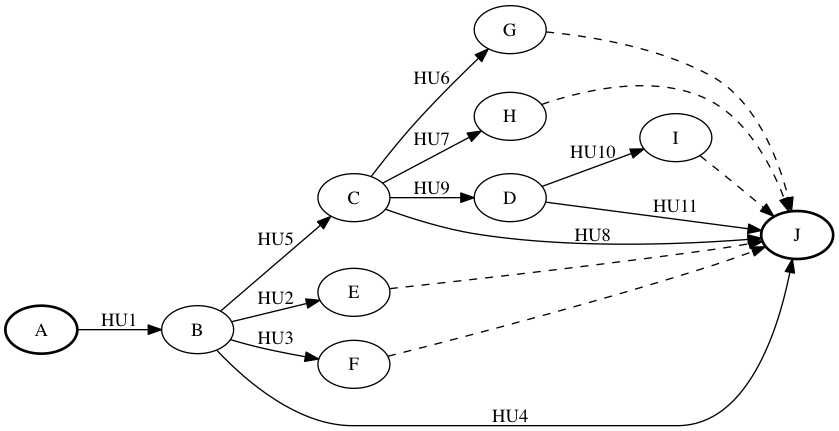
\includegraphics[width=\textwidth]{dependencies-graph}
			\caption{Modelo de dependencias del proyecto}\label{fig:dependencies}\index{Diagrama!de Descomposición Modular y Dependencias}
			\end{figure}
            
            \paragraph{}
            Como se puede observar, las historias de usuario\index{Historia de usuario}, ordenadas por el identificador numérico, sirven de referencia para tener una idea de dependencia entre estas. También se muestra el plan de evolución de la plataforma y la hoja de ruta que se quiere seguir para el desarrollo del proyecto\index{Proyecto!Desarrollo del}. Siendo determinante la primera historia de usuario para crear \textbf{elecciones}\index{Elección!Crear}, al ser el modelo principal sobre la que se basa la plataforma. Terminando por la visualización y reproducción del reparto de D'Hondt\index{D'Hondt!Reparto de}.

       	\subsection{Necesidades de recursos}
        
        	\paragraph{}
			Puesto que el modelo de proceso escogido para la realización de proyecto seguirá la metodología SCRUM\index{SCRUM} (en la cual se avanza en la ejecución del proyecto de manera iterativa, tratando obtener partes funcionales del sistema en cada una de las interacciones), se tratará de conseguir que la carga de recursos sea lo más homogénea posible. 
            
        	\paragraph{}
			Para cada historia de usuario\index{Historia de usuario} se dedicarán recursos para el análisis y diseño de la especificación completa de la misma, seguida de una fase de desarrollo de la interfaz gráfica y la funcionalidad. Además también se dedicarán recursos a la documentación de la misma.



       	\subsection{Presupuesto y asignación de recursos}

			\paragraph{}
            El proyecto no tiene financiación de ningún tipo, por lo que no se realizará una planificación de este tipo. La asignación de recursos\index{Proyecto!Recursos} de personal se distribuirá según la disponibilidad de cada uno de los miembros en cada periodo del proyecto.

       	\subsection{Planificación}

            \paragraph{}
			Se ha decidido dividir el trabajo en etapas de la misma duración (2 semanas). En SCRUM esto se denomina Sprint\index{SCRUM!Sprint}. Se realizarán 6 durante el desarrollo del proyecto agrupados en el siguiente rango de fechas:
            
            \begin{itemize}
            	\item \textbf{Sprint 1}: 17/10/2016 - 31/10/2016 

            	\item \textbf{Sprint 2}: 31/10/2016 - 14/11/2016

            	\item \textbf{Sprint 3}: 14/11/2016 - 28/11/2016

            	\item \textbf{Sprint 4}: 28/11/2016 - 12/12/2016

            	\item \textbf{Sprint 5}: 12/12/2016 - 26/12/2016

            	\item \textbf{Sprint 6}: 26/12/2016 - 09/01/2017

            \end{itemize}
			
            \paragraph{}
			Puesto que se seguirá la metodología SCRUM\index{SCRUM!Metodología} tan solo se planificará el primer Sprint\index{SCRUM!Sprint}. Una vez completado y con la experiencia adquirida se planificará el siguiente y así sucesivamente hasta la finalización del proyecto. Por lo tanto las historias de usuario del primer sprint son:
            
            \begin{itemize}
            	\item \textbf{\ref{itm:crear-eleccion}}: Historia de usuario\index{Historia de usuario} que en la creación de elecciones\index{Elección!Crear} en la plataforma mediante la interfaz. Esta historia de usuario nos ofrece un punto de partida para el desarrollo del proyecto\index{Proyecto!Desarrollo}, siendo las elecciones\index{Elección} la estructura central en la que se basa el resto de la plataforma. \newline El desarrollo de la tarea\index{Tarea} se tendrá tres principales partes:\begin{itemize}
            	\item Visualización
                \item Modelo
                
            	\end{itemize}

            	\item \textbf{\ref{itm:modificar-eleccion}}: Como ampliación de las primeras características que se consigan con el desarrollo de \ref{itm:crear-eleccion} esta historia de usuario\index{Historia de usuario} permitirá crear un patrón CRUD sobre estas. \newline Esta historia de usuario\index{Historia de usuario} permitirá la interacción entre el usuario pudiendo crear varias elecciones y modificándolas\index{Elección!Crear}\index{Elección!Modificar}, estableciendo las bases y dependencias para las siguientes etapas.

            \end{itemize}

	\clearpage
	\section{Componentes adicionales}
	    
        \paragraph{}
        Para el funcionamiento del proyecto podrán ser necesarios componentes adicionales que ayuden en su uso. Estos serán añadidos en esta sección del plan.
	\newpage
    \thispagestyle{fancy}
    \printindex
\end{document}
